\newpage
\section{Neural Networks}
A big part of this project revolved around artificial neural networks, which we used to model the distance maps of particular proteins. 
Therefore, in this section, we fully describe these neural networks.

We start by defining Perceptron, as the simplest instance of neural network architecture.
We show how the Perceptron is constructed, initialized and used to model mathematical functions.
Afterwards, we extend this neural network to enable it to model complex functions.
Next, we show how to use these networks to model spatially dependent data, like, for example, pictures.
Finally, we unite these theoretical concepts and reveal how we used them for the protein folding problem.

% Neural networks are machine learning models discovered in  
% In this section, we will present neural networks due to their high importance in the process of protein folding.

% With sufficient size, neural networks are able to learn any mathematical function.
% Their high complexity and flexibility even allows some particular subtypes, like for example recurrent neural networks, to be turing complete.

% The main challenge these systems are facing is in the fact, that they usually need very big datasets to learn the true mapping and training of such models on such big datasets are often infeasible.
% Nevertheless, the amounts of data collected by mankind is increasing and the computational resources are expected to increase as well. 

% Why Neural Networks?


\subsection{The basic architecture of Neural Networks}
Artificial neural networks are a machine learning models first discovered in 1958 by psychologist Frank Rosenblatt.
They were heavily inspired by the human nervous system.
The nervous system is composed of small units, called neurons.
These neurons are connected together via specialized connections called synapses.
The synaptic connections allow the neurons to send electrochemical signals to communicate with each another.
The strength of these connections regularly adapts to the external stimulation, which often changes the signal pathways and, in turn, influences the resulting reactions of the organism.
This process is commonly called learning.

\begin{figure}
    \centering
    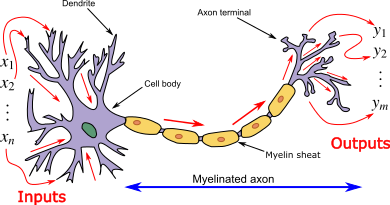
\includegraphics[width=0.5\linewidth]{imgs_andy/biological_neuron.png}
    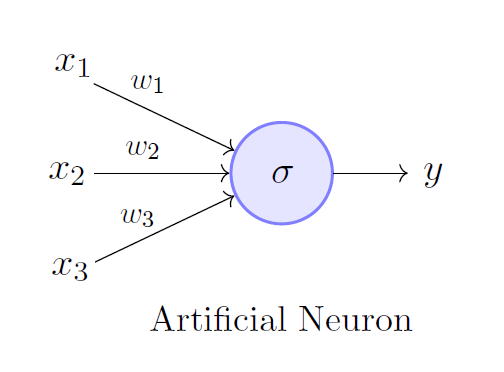
\includegraphics[width=0.5\linewidth]{imgs_andy/artificial_neuron.png}
    \caption{Biological  and Artificial neuron}
    \label{fig:neurons_comparison}
\end{figure}

In artificial neural networks, we simulate this process in a computer.
% from here it feels sloppy
Similarly to biological neural networks, in artificial neural networks we create multiple artificial neurons and initialize connections between them with some weights.
Then, we show an example of the input data, corresponding to external stimuli, to the network.
The network will produce some output value, which corresponds to the reaction of the organism.
Next, we compare this output value to our desired outcome and calculate the error made by our model.
Later, we adjust the weights of the connections in such a way, that the error is minimized.
We repeat this process until we are satisfied with the outputs from our neural network.

To formalize this process, we need to introduce some notation.
Let $X$ be an input to our network and let $Y$ be the desired output of our network.
Let us suppose, that there is a function $f: X \to Y$ which maps the input to our desired output.
Then, let us suppose, that our algorithm can generate some hypothesis $h$ from the hypothesis space $H$.
Now, we would like to approximate the function $f$ with such a hypothesis $h$, which produces the smallest possible error.

As an example, let us assume that we want to build a model, which is capable of distinguishing between cats and dogs.
We could collect many samples



Neural networks are composed of units called artificial neurons.
These neurons, similarly to biological neurons, are connected together to form the network.
Usually, the neurons are organized in layers, where each neuron in the layer $k$ is connected to each other neuron in the layer $k-1$.
Keywords: 
neuron, layer, pre-activation, activation function

Neural networks are machine learning methods inspired by the architecture of biological brains.
Similarly to the biological brains, the artificial neural networks consists of many neurons. 

\subsubsection{Parameter initialization}
\subsubsection{Forward pass}
\subsubsection{Backward pass}
Forward, Loss, Backward, parameter initialization
Activations
weights/parameters

\subsection{Convolutional Neural Networks}

\subsubsection{Convolution layers}
\subsubsection{Pooling layers}

\subsection{Residual Neural Networks}
    
\subsection{AlphaFold}
    